\chapter{System Design}

This chapter eludes on how the different components work together to create a working system.



\begin{figure}[h]
    \centering
    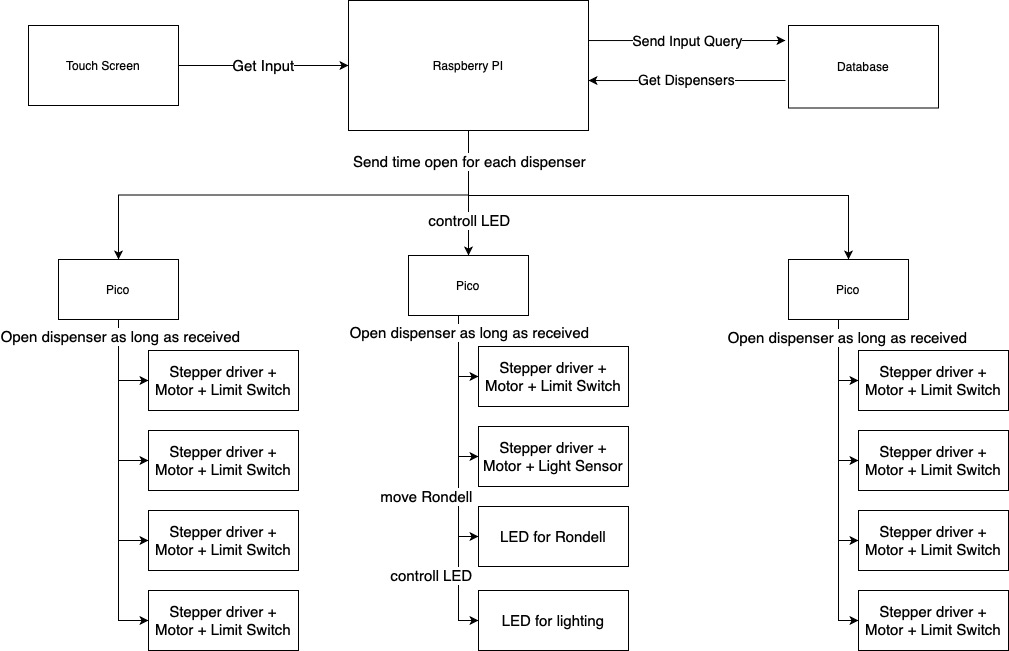
\includegraphics[width=140mm]{content/figures/overview.jpg}
    \caption{System overview\label{fig:overview}}
\end{figure}




\section{Communication}



\section{Sequence}

    When a beverage is selected on the touchscreen, the information about the beverage is queried in the database. With this information, the Main Controller sends the commands to the corresponding microcontrollers. The microcontrollers activate the corresponding stepper motor drives, which move the motor once the tap is open. After the time specified by the Main Controller, the dispenser is closed, so the motor reverses direction until the limit switch is closed, indicating that the motor is back in the neutral position.
